% Messung 365nm
\begin{table}
	\centering
	\begin{subtable}{0.5\textwidth}
		\centering
		\vspace{0pt}
		\resizebox{0.95\columnwidth}{!}{%
			\begin{tabular}{SSS}
	\toprule
	{$U$ / \si{\volt}} & {$I-I_0$ / \si{\nano\ampere}} & {$\Delta (I-I_0)$ / \si{\nano\ampere}} \\
	\midrule
0.001 & 18.522 & 0.373 \\
0.209 & 14.922 & 0.301 \\
0.397 & 11.122 & 0.225 \\
0.590 & 8.222  & 0.167 \\
0.793 & 5.422  & 0.111 \\
1.015 & 3.002  & 0.062 \\
1.203 & 1.652  & 0.035 \\
1.395 & 0.852  & 0.019 \\
1.595 & 0.342  & 0.009 \\
1.813 & 0.072  & 0.004 \\
1.997 & 0.022  & 0.003 \\
	\bottomrule
\end{tabular}

		}
		\caption{Messung 1}
	\end{subtable}%
	\begin{subtable}{0.5\textwidth}
		\centering
		\vspace{0pt}
		\resizebox{0.95\columnwidth}{!}{%
			\begin{tabular}{SSS}
	\toprule
	{$U$ / \si{\volt}} & {$I-I_0$ / \si{\nano\ampere}} & {$\Delta (I-I_0)$ / \si{\nano\ampere}} \\
	\midrule
0.001 & 18.927 & 0.381 \\
0.201 & 14.727 & 0.297 \\
0.400 & 11.327 & 0.229 \\
0.583 & 8.167  & 0.165 \\
0.790 & 5.347  & 0.109 \\
0.992 & 3.287  & 0.068 \\
1.185 & 1.817  & 0.038 \\
1.402 & 0.817  & 0.018 \\
1.595 & 0.337  & 0.009 \\
1.810 & 0.067  & 0.003 \\
2.016 & 0.027  & 0.003 \\
	\bottomrule
\end{tabular}

		}
		\caption{Messung 2}
	\end{subtable}

	\caption{Kennlinien der Photozelle f\"ur Licht der Wellenl\"ange $\lambda=\SI{365}{\nano\metre}$}
\end{table}

\begin{figure}
	\centering
	% GNUPLOT: LaTeX picture with Postscript
\begingroup
  \makeatletter
  \providecommand\color[2][]{%
    \GenericError{(gnuplot) \space\space\space\@spaces}{%
      Package color not loaded in conjunction with
      terminal option `colourtext'%
    }{See the gnuplot documentation for explanation.%
    }{Either use 'blacktext' in gnuplot or load the package
      color.sty in LaTeX.}%
    \renewcommand\color[2][]{}%
  }%
  \providecommand\includegraphics[2][]{%
    \GenericError{(gnuplot) \space\space\space\@spaces}{%
      Package graphicx or graphics not loaded%
    }{See the gnuplot documentation for explanation.%
    }{The gnuplot epslatex terminal needs graphicx.sty or graphics.sty.}%
    \renewcommand\includegraphics[2][]{}%
  }%
  \providecommand\rotatebox[2]{#2}%
  \@ifundefined{ifGPcolor}{%
    \newif\ifGPcolor
    \GPcolortrue
  }{}%
  \@ifundefined{ifGPblacktext}{%
    \newif\ifGPblacktext
    \GPblacktexttrue
  }{}%
  % define a \g@addto@macro without @ in the name:
  \let\gplgaddtomacro\g@addto@macro
  % define empty templates for all commands taking text:
  \gdef\gplbacktext{}%
  \gdef\gplfronttext{}%
  \makeatother
  \ifGPblacktext
    % no textcolor at all
    \def\colorrgb#1{}%
    \def\colorgray#1{}%
  \else
    % gray or color?
    \ifGPcolor
      \def\colorrgb#1{\color[rgb]{#1}}%
      \def\colorgray#1{\color[gray]{#1}}%
      \expandafter\def\csname LTw\endcsname{\color{white}}%
      \expandafter\def\csname LTb\endcsname{\color{black}}%
      \expandafter\def\csname LTa\endcsname{\color{black}}%
      \expandafter\def\csname LT0\endcsname{\color[rgb]{1,0,0}}%
      \expandafter\def\csname LT1\endcsname{\color[rgb]{0,1,0}}%
      \expandafter\def\csname LT2\endcsname{\color[rgb]{0,0,1}}%
      \expandafter\def\csname LT3\endcsname{\color[rgb]{1,0,1}}%
      \expandafter\def\csname LT4\endcsname{\color[rgb]{0,1,1}}%
      \expandafter\def\csname LT5\endcsname{\color[rgb]{1,1,0}}%
      \expandafter\def\csname LT6\endcsname{\color[rgb]{0,0,0}}%
      \expandafter\def\csname LT7\endcsname{\color[rgb]{1,0.3,0}}%
      \expandafter\def\csname LT8\endcsname{\color[rgb]{0.5,0.5,0.5}}%
    \else
      % gray
      \def\colorrgb#1{\color{black}}%
      \def\colorgray#1{\color[gray]{#1}}%
      \expandafter\def\csname LTw\endcsname{\color{white}}%
      \expandafter\def\csname LTb\endcsname{\color{black}}%
      \expandafter\def\csname LTa\endcsname{\color{black}}%
      \expandafter\def\csname LT0\endcsname{\color{black}}%
      \expandafter\def\csname LT1\endcsname{\color{black}}%
      \expandafter\def\csname LT2\endcsname{\color{black}}%
      \expandafter\def\csname LT3\endcsname{\color{black}}%
      \expandafter\def\csname LT4\endcsname{\color{black}}%
      \expandafter\def\csname LT5\endcsname{\color{black}}%
      \expandafter\def\csname LT6\endcsname{\color{black}}%
      \expandafter\def\csname LT7\endcsname{\color{black}}%
      \expandafter\def\csname LT8\endcsname{\color{black}}%
    \fi
  \fi
  \setlength{\unitlength}{0.0500bp}%
  \begin{picture}(6480.00,4320.00)%
    \gplgaddtomacro\gplbacktext{%
      \csname LTb\endcsname%
      \put(946,704){\makebox(0,0)[r]{\strut{} 0}}%
      \csname LTb\endcsname%
      \put(946,1076){\makebox(0,0)[r]{\strut{} 0,5}}%
      \csname LTb\endcsname%
      \put(946,1449){\makebox(0,0)[r]{\strut{} 1}}%
      \csname LTb\endcsname%
      \put(946,1821){\makebox(0,0)[r]{\strut{} 1,5}}%
      \csname LTb\endcsname%
      \put(946,2193){\makebox(0,0)[r]{\strut{} 2}}%
      \csname LTb\endcsname%
      \put(946,2566){\makebox(0,0)[r]{\strut{} 2,5}}%
      \csname LTb\endcsname%
      \put(946,2938){\makebox(0,0)[r]{\strut{} 3}}%
      \csname LTb\endcsname%
      \put(946,3310){\makebox(0,0)[r]{\strut{} 3,5}}%
      \csname LTb\endcsname%
      \put(946,3683){\makebox(0,0)[r]{\strut{} 4}}%
      \csname LTb\endcsname%
      \put(946,4055){\makebox(0,0)[r]{\strut{} 4,5}}%
      \csname LTb\endcsname%
      \put(1078,484){\makebox(0,0){\strut{} 0}}%
      \csname LTb\endcsname%
      \put(2079,484){\makebox(0,0){\strut{} 0,5}}%
      \csname LTb\endcsname%
      \put(3080,484){\makebox(0,0){\strut{} 1}}%
      \csname LTb\endcsname%
      \put(4081,484){\makebox(0,0){\strut{} 1,5}}%
      \csname LTb\endcsname%
      \put(5082,484){\makebox(0,0){\strut{} 2}}%
      \csname LTb\endcsname%
      \put(6083,484){\makebox(0,0){\strut{} 2,5}}%
      \put(176,2379){\rotatebox{-270}{\makebox(0,0){\strut{}$\sqrt{I-I_0} \, / \, \si{\nano\ampere^{1/2}}$}}}%
      \put(3580,154){\makebox(0,0){\strut{}$U \, / \, \si{\volt}$}}%
      \put(3580,3945){\makebox(0,0){\strut{}}}%
    }%
    \gplgaddtomacro\gplfronttext{%
      \csname LTb\endcsname%
      \put(5096,3882){\makebox(0,0)[r]{\strut{}Messung 1}}%
      \csname LTb\endcsname%
      \put(5096,3662){\makebox(0,0)[r]{\strut{}Regressionsgerade 1}}%
      \csname LTb\endcsname%
      \put(5096,3442){\makebox(0,0)[r]{\strut{}Messung 2}}%
      \csname LTb\endcsname%
      \put(5096,3222){\makebox(0,0)[r]{\strut{}Regressionsgerade 2}}%
    }%
    \gplbacktext
    \put(0,0){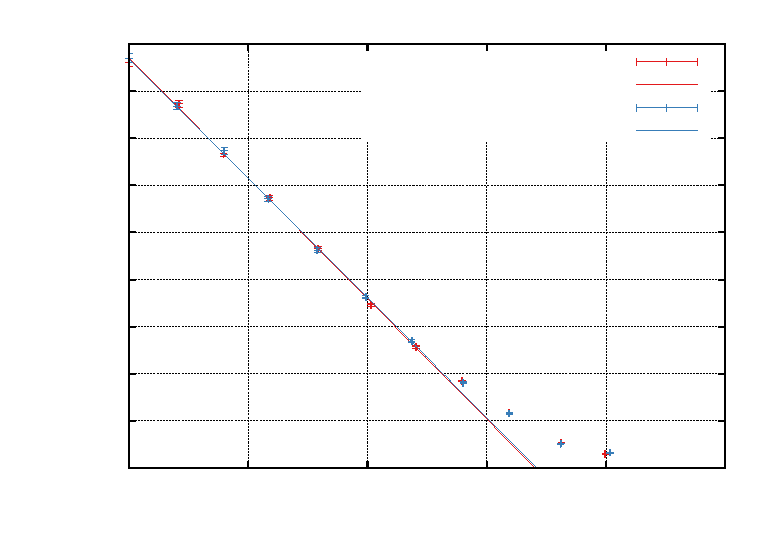
\includegraphics{./plots/photo/kennlinien_365nm}}%
    \gplfronttext
  \end{picture}%
\endgroup

	\caption{Kennlinien 365nm}
	\label{fig:kennlinien_365nm}
\end{figure}



% Messung 405nm
\begin{table}
	\centering
	\begin{subtable}{0.5\textwidth}
		\centering
		\vspace{0pt}
		\resizebox{0.95\columnwidth}{!}{%
			\begin{tabular}{SSS}
	\toprule
	{$U$ / \si{\volt}} & {$I-I_0$ / \si{\nano\ampere}} & {$\Delta (I-I_0)$ / \si{\nano\ampere}} \\
	\midrule
0.001 & 7.714 & 0.157 \\
0.156 & 6.164 & 0.126 \\
0.315 & 4.784 & 0.098 \\
0.452 & 3.634 & 0.075 \\
0.611 & 2.484 & 0.052 \\
0.745 & 1.684 & 0.036 \\
0.913 & 0.914 & 0.021 \\
1.053 & 0.544 & 0.013 \\
1.189 & 0.304 & 0.008 \\
1.346 & 0.104 & 0.004 \\
1.494 & 0.024 & 0.003 \\
1.632 & 0.004 & 0.003 \\
	\bottomrule
\end{tabular}

		}
		\caption{Messung 1}
	\end{subtable}%
	\begin{subtable}{0.5\textwidth}
		\centering
		\vspace{0pt}
		\resizebox{0.95\columnwidth}{!}{%
			\begin{tabular}{SSS}
	\toprule
	{$U$ / \si{\volt}} & {$I-I_0$ / \si{\nano\ampere}} & {$\Delta (I-I_0)$ / \si{\nano\ampere}} \\
	\midrule
0.001 & 7.661 & 0.155 \\
0.132 & 6.321 & 0.129 \\
0.318 & 4.721 & 0.097 \\
0.447 & 3.651 & 0.075 \\
0.598 & 2.571 & 0.054 \\
0.753 & 1.641 & 0.035 \\
0.896 & 0.991 & 0.022 \\
1.038 & 0.571 & 0.014 \\
1.189 & 0.301 & 0.008 \\
1.349 & 0.111 & 0.004 \\
1.487 & 0.031 & 0.003 \\
	\bottomrule
\end{tabular}


		}
		\caption{Messung 2}
	\end{subtable}

	\caption{Kennlinien der Photozelle f\"ur Licht der Wellenl\"ange $\lambda = \SI{405}{\nano\metre}$}
\end{table}

\begin{figure}
	\centering
	% GNUPLOT: LaTeX picture with Postscript
\begingroup
  \makeatletter
  \providecommand\color[2][]{%
    \GenericError{(gnuplot) \space\space\space\@spaces}{%
      Package color not loaded in conjunction with
      terminal option `colourtext'%
    }{See the gnuplot documentation for explanation.%
    }{Either use 'blacktext' in gnuplot or load the package
      color.sty in LaTeX.}%
    \renewcommand\color[2][]{}%
  }%
  \providecommand\includegraphics[2][]{%
    \GenericError{(gnuplot) \space\space\space\@spaces}{%
      Package graphicx or graphics not loaded%
    }{See the gnuplot documentation for explanation.%
    }{The gnuplot epslatex terminal needs graphicx.sty or graphics.sty.}%
    \renewcommand\includegraphics[2][]{}%
  }%
  \providecommand\rotatebox[2]{#2}%
  \@ifundefined{ifGPcolor}{%
    \newif\ifGPcolor
    \GPcolortrue
  }{}%
  \@ifundefined{ifGPblacktext}{%
    \newif\ifGPblacktext
    \GPblacktexttrue
  }{}%
  % define a \g@addto@macro without @ in the name:
  \let\gplgaddtomacro\g@addto@macro
  % define empty templates for all commands taking text:
  \gdef\gplbacktext{}%
  \gdef\gplfronttext{}%
  \makeatother
  \ifGPblacktext
    % no textcolor at all
    \def\colorrgb#1{}%
    \def\colorgray#1{}%
  \else
    % gray or color?
    \ifGPcolor
      \def\colorrgb#1{\color[rgb]{#1}}%
      \def\colorgray#1{\color[gray]{#1}}%
      \expandafter\def\csname LTw\endcsname{\color{white}}%
      \expandafter\def\csname LTb\endcsname{\color{black}}%
      \expandafter\def\csname LTa\endcsname{\color{black}}%
      \expandafter\def\csname LT0\endcsname{\color[rgb]{1,0,0}}%
      \expandafter\def\csname LT1\endcsname{\color[rgb]{0,1,0}}%
      \expandafter\def\csname LT2\endcsname{\color[rgb]{0,0,1}}%
      \expandafter\def\csname LT3\endcsname{\color[rgb]{1,0,1}}%
      \expandafter\def\csname LT4\endcsname{\color[rgb]{0,1,1}}%
      \expandafter\def\csname LT5\endcsname{\color[rgb]{1,1,0}}%
      \expandafter\def\csname LT6\endcsname{\color[rgb]{0,0,0}}%
      \expandafter\def\csname LT7\endcsname{\color[rgb]{1,0.3,0}}%
      \expandafter\def\csname LT8\endcsname{\color[rgb]{0.5,0.5,0.5}}%
    \else
      % gray
      \def\colorrgb#1{\color{black}}%
      \def\colorgray#1{\color[gray]{#1}}%
      \expandafter\def\csname LTw\endcsname{\color{white}}%
      \expandafter\def\csname LTb\endcsname{\color{black}}%
      \expandafter\def\csname LTa\endcsname{\color{black}}%
      \expandafter\def\csname LT0\endcsname{\color{black}}%
      \expandafter\def\csname LT1\endcsname{\color{black}}%
      \expandafter\def\csname LT2\endcsname{\color{black}}%
      \expandafter\def\csname LT3\endcsname{\color{black}}%
      \expandafter\def\csname LT4\endcsname{\color{black}}%
      \expandafter\def\csname LT5\endcsname{\color{black}}%
      \expandafter\def\csname LT6\endcsname{\color{black}}%
      \expandafter\def\csname LT7\endcsname{\color{black}}%
      \expandafter\def\csname LT8\endcsname{\color{black}}%
    \fi
  \fi
  \setlength{\unitlength}{0.0500bp}%
  \begin{picture}(7200.00,5040.00)%
    \gplgaddtomacro\gplbacktext{%
      \csname LTb\endcsname%
      \put(946,704){\makebox(0,0)[r]{\strut{} 0}}%
      \csname LTb\endcsname%
      \put(946,1383){\makebox(0,0)[r]{\strut{} 0.5}}%
      \csname LTb\endcsname%
      \put(946,2061){\makebox(0,0)[r]{\strut{} 1}}%
      \csname LTb\endcsname%
      \put(946,2740){\makebox(0,0)[r]{\strut{} 1.5}}%
      \csname LTb\endcsname%
      \put(946,3418){\makebox(0,0)[r]{\strut{} 2}}%
      \csname LTb\endcsname%
      \put(946,4097){\makebox(0,0)[r]{\strut{} 2.5}}%
      \csname LTb\endcsname%
      \put(946,4775){\makebox(0,0)[r]{\strut{} 3}}%
      \csname LTb\endcsname%
      \put(1078,484){\makebox(0,0){\strut{} 0}}%
      \csname LTb\endcsname%
      \put(1714,484){\makebox(0,0){\strut{} 0.2}}%
      \csname LTb\endcsname%
      \put(2350,484){\makebox(0,0){\strut{} 0.4}}%
      \csname LTb\endcsname%
      \put(2986,484){\makebox(0,0){\strut{} 0.6}}%
      \csname LTb\endcsname%
      \put(3622,484){\makebox(0,0){\strut{} 0.8}}%
      \csname LTb\endcsname%
      \put(4259,484){\makebox(0,0){\strut{} 1}}%
      \csname LTb\endcsname%
      \put(4895,484){\makebox(0,0){\strut{} 1.2}}%
      \csname LTb\endcsname%
      \put(5531,484){\makebox(0,0){\strut{} 1.4}}%
      \csname LTb\endcsname%
      \put(6167,484){\makebox(0,0){\strut{} 1.6}}%
      \csname LTb\endcsname%
      \put(6803,484){\makebox(0,0){\strut{} 1.8}}%
      \put(176,2739){\rotatebox{-270}{\makebox(0,0){\strut{}$\sqrt{I-I_0} \, / \, \si{\nano\ampere^{1/2}}$}}}%
      \put(3940,154){\makebox(0,0){\strut{}$U \, / \, \si{\volt}$}}%
      \put(3940,4665){\makebox(0,0){\strut{}}}%
    }%
    \gplgaddtomacro\gplfronttext{%
      \csname LTb\endcsname%
      \put(5816,4602){\makebox(0,0)[r]{\strut{}Messung 1}}%
      \csname LTb\endcsname%
      \put(5816,4382){\makebox(0,0)[r]{\strut{}Regressionsgerade 1}}%
      \csname LTb\endcsname%
      \put(5816,4162){\makebox(0,0)[r]{\strut{}Messung 2}}%
      \csname LTb\endcsname%
      \put(5816,3942){\makebox(0,0)[r]{\strut{}Regressionsgerade 2}}%
    }%
    \gplbacktext
    \put(0,0){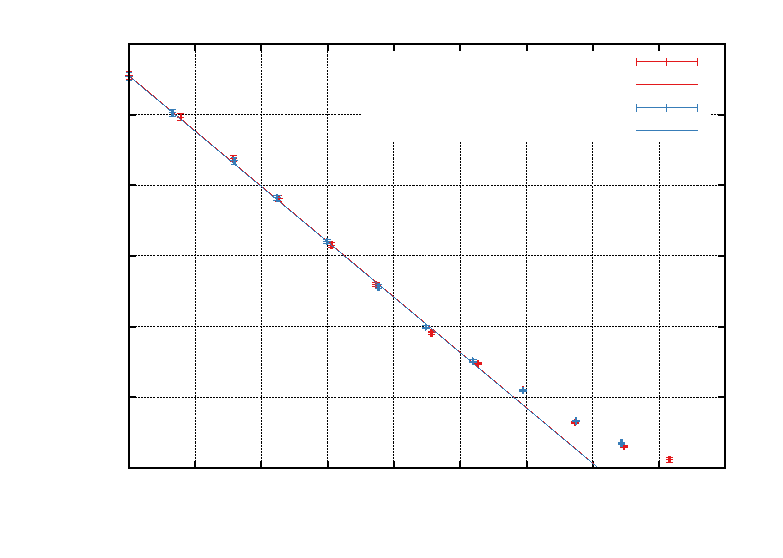
\includegraphics{./plots/photo/kennlinien_405nm}}%
    \gplfronttext
  \end{picture}%
\endgroup

	\caption{Kennlinien 405nm}
	\label{fig:kennlinien_405nm}
\end{figure}



% Messung 436nm
\begin{table}
	\centering
	\begin{subtable}{0.5\textwidth}
		\centering
		\vspace{0pt}
		\resizebox{0.95\columnwidth}{!}{%
			\begin{tabular}{SSS}
	\toprule
	{$U$ / \si{\volt}} & {$I-I_0$ / \si{\nano\ampere}} & {$\Delta (I-I_0)$ / \si{\nano\ampere}} \\
	\midrule
0.001 & 13.120 & 0.265 \\
0.091 & 11.708 & 0.237 \\
0.204 & 9.328  & 0.189 \\
0.289 & 7.808  & 0.159 \\
0.401 & 5.958  & 0.122 \\
0.510 & 4.608  & 0.095 \\
0.604 & 3.428  & 0.071 \\
0.700 & 2.338  & 0.049 \\
0.802 & 1.498  & 0.032 \\
0.894 & 0.988  & 0.022 \\
0.993 & 0.628  & 0.015 \\
1.102 & 0.318  & 0.009 \\
1.201 & 0.108  & 0.005 \\
1.306 & 0.028  & 0.003 \\
1.405 & 0.008  & 0.003 \\
	\bottomrule
\end{tabular}

		}
		\caption{Messung 1}
	\end{subtable}%
	\begin{subtable}{0.5\textwidth}
		\centering
		\vspace{0pt}
		\resizebox{0.95\columnwidth}{!}{%
			\begin{tabular}{SSS}
	\toprule
	{$U$ / \si{\volt}} & {$I-I_0$ / \si{\nano\ampere}} & {$\Delta (I-I_0)$ / \si{\nano\ampere}} \\
	\midrule
0.001 & 13.372 & 0.270 \\
0.103 & 11.522 & 0.233 \\
0.199 & 9.712  & 0.196 \\
0.311 & 7.622  & 0.155 \\
0.405 & 5.942  & 0.121 \\
0.508 & 4.482  & 0.092 \\
0.593 & 3.432  & 0.071 \\
0.705 & 2.262  & 0.047 \\
0.801 & 1.512  & 0.032 \\
0.904 & 0.962  & 0.021 \\
0.998 & 0.622  & 0.015 \\
1.106 & 0.312  & 0.008 \\
1.205 & 0.112  & 0.004 \\
1.291 & 0.042  & 0.003 \\
	\bottomrule
\end{tabular}

		}
		\caption{Messung 2}
	\end{subtable}

	\caption{Kennlinien der Photozelle f\"ur Licht der Wellenl\"ange $\lambda = \SI{436}{\nano\metre}$}
\end{table}

\begin{figure}
	\centering
	% GNUPLOT: LaTeX picture with Postscript
\begingroup
  \makeatletter
  \providecommand\color[2][]{%
    \GenericError{(gnuplot) \space\space\space\@spaces}{%
      Package color not loaded in conjunction with
      terminal option `colourtext'%
    }{See the gnuplot documentation for explanation.%
    }{Either use 'blacktext' in gnuplot or load the package
      color.sty in LaTeX.}%
    \renewcommand\color[2][]{}%
  }%
  \providecommand\includegraphics[2][]{%
    \GenericError{(gnuplot) \space\space\space\@spaces}{%
      Package graphicx or graphics not loaded%
    }{See the gnuplot documentation for explanation.%
    }{The gnuplot epslatex terminal needs graphicx.sty or graphics.sty.}%
    \renewcommand\includegraphics[2][]{}%
  }%
  \providecommand\rotatebox[2]{#2}%
  \@ifundefined{ifGPcolor}{%
    \newif\ifGPcolor
    \GPcolortrue
  }{}%
  \@ifundefined{ifGPblacktext}{%
    \newif\ifGPblacktext
    \GPblacktexttrue
  }{}%
  % define a \g@addto@macro without @ in the name:
  \let\gplgaddtomacro\g@addto@macro
  % define empty templates for all commands taking text:
  \gdef\gplbacktext{}%
  \gdef\gplfronttext{}%
  \makeatother
  \ifGPblacktext
    % no textcolor at all
    \def\colorrgb#1{}%
    \def\colorgray#1{}%
  \else
    % gray or color?
    \ifGPcolor
      \def\colorrgb#1{\color[rgb]{#1}}%
      \def\colorgray#1{\color[gray]{#1}}%
      \expandafter\def\csname LTw\endcsname{\color{white}}%
      \expandafter\def\csname LTb\endcsname{\color{black}}%
      \expandafter\def\csname LTa\endcsname{\color{black}}%
      \expandafter\def\csname LT0\endcsname{\color[rgb]{1,0,0}}%
      \expandafter\def\csname LT1\endcsname{\color[rgb]{0,1,0}}%
      \expandafter\def\csname LT2\endcsname{\color[rgb]{0,0,1}}%
      \expandafter\def\csname LT3\endcsname{\color[rgb]{1,0,1}}%
      \expandafter\def\csname LT4\endcsname{\color[rgb]{0,1,1}}%
      \expandafter\def\csname LT5\endcsname{\color[rgb]{1,1,0}}%
      \expandafter\def\csname LT6\endcsname{\color[rgb]{0,0,0}}%
      \expandafter\def\csname LT7\endcsname{\color[rgb]{1,0.3,0}}%
      \expandafter\def\csname LT8\endcsname{\color[rgb]{0.5,0.5,0.5}}%
    \else
      % gray
      \def\colorrgb#1{\color{black}}%
      \def\colorgray#1{\color[gray]{#1}}%
      \expandafter\def\csname LTw\endcsname{\color{white}}%
      \expandafter\def\csname LTb\endcsname{\color{black}}%
      \expandafter\def\csname LTa\endcsname{\color{black}}%
      \expandafter\def\csname LT0\endcsname{\color{black}}%
      \expandafter\def\csname LT1\endcsname{\color{black}}%
      \expandafter\def\csname LT2\endcsname{\color{black}}%
      \expandafter\def\csname LT3\endcsname{\color{black}}%
      \expandafter\def\csname LT4\endcsname{\color{black}}%
      \expandafter\def\csname LT5\endcsname{\color{black}}%
      \expandafter\def\csname LT6\endcsname{\color{black}}%
      \expandafter\def\csname LT7\endcsname{\color{black}}%
      \expandafter\def\csname LT8\endcsname{\color{black}}%
    \fi
  \fi
  \setlength{\unitlength}{0.0500bp}%
  \begin{picture}(7200.00,5040.00)%
    \gplgaddtomacro\gplbacktext{%
      \csname LTb\endcsname%
      \put(946,704){\makebox(0,0)[r]{\strut{} 0}}%
      \csname LTb\endcsname%
      \put(946,1213){\makebox(0,0)[r]{\strut{} 0.5}}%
      \csname LTb\endcsname%
      \put(946,1722){\makebox(0,0)[r]{\strut{} 1}}%
      \csname LTb\endcsname%
      \put(946,2231){\makebox(0,0)[r]{\strut{} 1.5}}%
      \csname LTb\endcsname%
      \put(946,2740){\makebox(0,0)[r]{\strut{} 2}}%
      \csname LTb\endcsname%
      \put(946,3248){\makebox(0,0)[r]{\strut{} 2.5}}%
      \csname LTb\endcsname%
      \put(946,3757){\makebox(0,0)[r]{\strut{} 3}}%
      \csname LTb\endcsname%
      \put(946,4266){\makebox(0,0)[r]{\strut{} 3.5}}%
      \csname LTb\endcsname%
      \put(946,4775){\makebox(0,0)[r]{\strut{} 4}}%
      \csname LTb\endcsname%
      \put(1078,484){\makebox(0,0){\strut{} 0}}%
      \csname LTb\endcsname%
      \put(1794,484){\makebox(0,0){\strut{} 0.2}}%
      \csname LTb\endcsname%
      \put(2509,484){\makebox(0,0){\strut{} 0.4}}%
      \csname LTb\endcsname%
      \put(3225,484){\makebox(0,0){\strut{} 0.6}}%
      \csname LTb\endcsname%
      \put(3941,484){\makebox(0,0){\strut{} 0.8}}%
      \csname LTb\endcsname%
      \put(4656,484){\makebox(0,0){\strut{} 1}}%
      \csname LTb\endcsname%
      \put(5372,484){\makebox(0,0){\strut{} 1.2}}%
      \csname LTb\endcsname%
      \put(6087,484){\makebox(0,0){\strut{} 1.4}}%
      \csname LTb\endcsname%
      \put(6803,484){\makebox(0,0){\strut{} 1.6}}%
      \put(176,2739){\rotatebox{-270}{\makebox(0,0){\strut{}$\sqrt{I-I_0} \, / \, \si{\nano\ampere^{1/2}}$}}}%
      \put(3940,154){\makebox(0,0){\strut{}$U \, / \, \si{\volt}$}}%
      \put(3940,4665){\makebox(0,0){\strut{}}}%
    }%
    \gplgaddtomacro\gplfronttext{%
      \csname LTb\endcsname%
      \put(5816,4602){\makebox(0,0)[r]{\strut{}Messung 1}}%
      \csname LTb\endcsname%
      \put(5816,4382){\makebox(0,0)[r]{\strut{}Regressionsgerade 1}}%
      \csname LTb\endcsname%
      \put(5816,4162){\makebox(0,0)[r]{\strut{}Messung 2}}%
      \csname LTb\endcsname%
      \put(5816,3942){\makebox(0,0)[r]{\strut{}Regressionsgerade 2}}%
    }%
    \gplbacktext
    \put(0,0){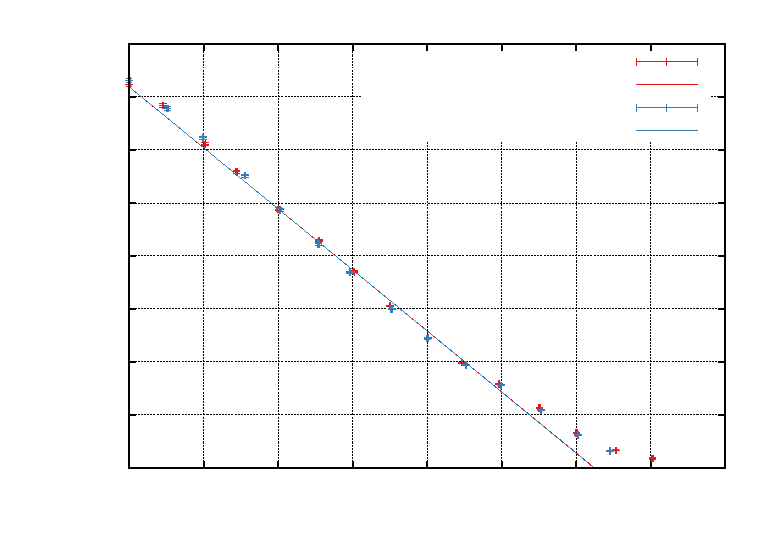
\includegraphics{./plots/photo/kennlinien_436nm}}%
    \gplfronttext
  \end{picture}%
\endgroup

	\caption{Kennlinien 436nm}
	\label{fig:kennlinien_436nm}
\end{figure}



% Messung 546nm
\begin{table}
	\centering
	\begin{subtable}{0.5\textwidth}
		\centering
		\vspace{0pt}
		\resizebox{0.95\columnwidth}{!}{%
			\begin{tabular}{SSS}
	\toprule
	{$U$ / \si{\volt}} & {$I-I_0$ / \si{\nano\ampere}} & {$\Delta (I-I_0)$ / \si{\nano\ampere}} \\
	\midrule
0.001 & 10.261 & 0.208 \\
0.073 & 8.261  & 0.168 \\
0.150 & 6.331  & 0.129 \\
0.225 & 4.771  & 0.098 \\
0.301 & 3.371  & 0.070 \\
0.376 & 2.221  & 0.047 \\
0.448 & 1.371  & 0.030 \\
0.533 & 0.721  & 0.017 \\
0.609 & 0.371  & 0.010 \\
0.673 & 0.201  & 0.006 \\
0.754 & 0.051  & 0.003 \\
0.838 & 0.001  & 0.003 \\
	\bottomrule
\end{tabular}

		}
		\caption{Messung 1}
	\end{subtable}%
	\begin{subtable}{0.5\textwidth}
		\centering
		\vspace{0pt}
		\resizebox{0.95\columnwidth}{!}{%
			\begin{tabular}{SSS}
	\toprule
	{$U$ / \si{\volt}} & {$I-I_0$ / \si{\nano\ampere}} & {$\Delta (I-I_0)$ / \si{\nano\ampere}} \\
	\midrule
0.001 & 10.185 & 0.206 \\
0.067 & 8.405  & 0.170 \\
0.166 & 6.035  & 0.123 \\
0.230 & 4.675  & 0.096 \\
0.300 & 3.385  & 0.070 \\
0.379 & 2.185  & 0.046 \\
0.450 & 1.425  & 0.031 \\
0.527 & 0.775  & 0.018 \\
0.594 & 0.415  & 0.011 \\
0.661 & 0.235  & 0.007 \\
0.765 & 0.045  & 0.003 \\
 & & \\
	\bottomrule
\end{tabular}

		}
		\caption{Messung 2}
	\end{subtable}

	\caption{Kennlinien der Photozelle f\"ur Licht der Wellenl\"ange $\lambda = \SI{546}{\nano\metre}$}
\end{table}

\begin{figure}
	\centering
	% GNUPLOT: LaTeX picture with Postscript
\begingroup
  \makeatletter
  \providecommand\color[2][]{%
    \GenericError{(gnuplot) \space\space\space\@spaces}{%
      Package color not loaded in conjunction with
      terminal option `colourtext'%
    }{See the gnuplot documentation for explanation.%
    }{Either use 'blacktext' in gnuplot or load the package
      color.sty in LaTeX.}%
    \renewcommand\color[2][]{}%
  }%
  \providecommand\includegraphics[2][]{%
    \GenericError{(gnuplot) \space\space\space\@spaces}{%
      Package graphicx or graphics not loaded%
    }{See the gnuplot documentation for explanation.%
    }{The gnuplot epslatex terminal needs graphicx.sty or graphics.sty.}%
    \renewcommand\includegraphics[2][]{}%
  }%
  \providecommand\rotatebox[2]{#2}%
  \@ifundefined{ifGPcolor}{%
    \newif\ifGPcolor
    \GPcolortrue
  }{}%
  \@ifundefined{ifGPblacktext}{%
    \newif\ifGPblacktext
    \GPblacktexttrue
  }{}%
  % define a \g@addto@macro without @ in the name:
  \let\gplgaddtomacro\g@addto@macro
  % define empty templates for all commands taking text:
  \gdef\gplbacktext{}%
  \gdef\gplfronttext{}%
  \makeatother
  \ifGPblacktext
    % no textcolor at all
    \def\colorrgb#1{}%
    \def\colorgray#1{}%
  \else
    % gray or color?
    \ifGPcolor
      \def\colorrgb#1{\color[rgb]{#1}}%
      \def\colorgray#1{\color[gray]{#1}}%
      \expandafter\def\csname LTw\endcsname{\color{white}}%
      \expandafter\def\csname LTb\endcsname{\color{black}}%
      \expandafter\def\csname LTa\endcsname{\color{black}}%
      \expandafter\def\csname LT0\endcsname{\color[rgb]{1,0,0}}%
      \expandafter\def\csname LT1\endcsname{\color[rgb]{0,1,0}}%
      \expandafter\def\csname LT2\endcsname{\color[rgb]{0,0,1}}%
      \expandafter\def\csname LT3\endcsname{\color[rgb]{1,0,1}}%
      \expandafter\def\csname LT4\endcsname{\color[rgb]{0,1,1}}%
      \expandafter\def\csname LT5\endcsname{\color[rgb]{1,1,0}}%
      \expandafter\def\csname LT6\endcsname{\color[rgb]{0,0,0}}%
      \expandafter\def\csname LT7\endcsname{\color[rgb]{1,0.3,0}}%
      \expandafter\def\csname LT8\endcsname{\color[rgb]{0.5,0.5,0.5}}%
    \else
      % gray
      \def\colorrgb#1{\color{black}}%
      \def\colorgray#1{\color[gray]{#1}}%
      \expandafter\def\csname LTw\endcsname{\color{white}}%
      \expandafter\def\csname LTb\endcsname{\color{black}}%
      \expandafter\def\csname LTa\endcsname{\color{black}}%
      \expandafter\def\csname LT0\endcsname{\color{black}}%
      \expandafter\def\csname LT1\endcsname{\color{black}}%
      \expandafter\def\csname LT2\endcsname{\color{black}}%
      \expandafter\def\csname LT3\endcsname{\color{black}}%
      \expandafter\def\csname LT4\endcsname{\color{black}}%
      \expandafter\def\csname LT5\endcsname{\color{black}}%
      \expandafter\def\csname LT6\endcsname{\color{black}}%
      \expandafter\def\csname LT7\endcsname{\color{black}}%
      \expandafter\def\csname LT8\endcsname{\color{black}}%
    \fi
  \fi
  \setlength{\unitlength}{0.0500bp}%
  \begin{picture}(7200.00,5040.00)%
    \gplgaddtomacro\gplbacktext{%
      \csname LTb\endcsname%
      \put(946,704){\makebox(0,0)[r]{\strut{} 0}}%
      \csname LTb\endcsname%
      \put(946,1286){\makebox(0,0)[r]{\strut{} 0.5}}%
      \csname LTb\endcsname%
      \put(946,1867){\makebox(0,0)[r]{\strut{} 1}}%
      \csname LTb\endcsname%
      \put(946,2449){\makebox(0,0)[r]{\strut{} 1.5}}%
      \csname LTb\endcsname%
      \put(946,3030){\makebox(0,0)[r]{\strut{} 2}}%
      \csname LTb\endcsname%
      \put(946,3612){\makebox(0,0)[r]{\strut{} 2.5}}%
      \csname LTb\endcsname%
      \put(946,4193){\makebox(0,0)[r]{\strut{} 3}}%
      \csname LTb\endcsname%
      \put(946,4775){\makebox(0,0)[r]{\strut{} 3.5}}%
      \csname LTb\endcsname%
      \put(1078,484){\makebox(0,0){\strut{} 0}}%
      \csname LTb\endcsname%
      \put(1714,484){\makebox(0,0){\strut{} 0.1}}%
      \csname LTb\endcsname%
      \put(2350,484){\makebox(0,0){\strut{} 0.2}}%
      \csname LTb\endcsname%
      \put(2986,484){\makebox(0,0){\strut{} 0.3}}%
      \csname LTb\endcsname%
      \put(3622,484){\makebox(0,0){\strut{} 0.4}}%
      \csname LTb\endcsname%
      \put(4259,484){\makebox(0,0){\strut{} 0.5}}%
      \csname LTb\endcsname%
      \put(4895,484){\makebox(0,0){\strut{} 0.6}}%
      \csname LTb\endcsname%
      \put(5531,484){\makebox(0,0){\strut{} 0.7}}%
      \csname LTb\endcsname%
      \put(6167,484){\makebox(0,0){\strut{} 0.8}}%
      \csname LTb\endcsname%
      \put(6803,484){\makebox(0,0){\strut{} 0.9}}%
      \put(176,2739){\rotatebox{-270}{\makebox(0,0){\strut{}$\sqrt{I-I_0} \, / \, \si{\nano\ampere^{1/2}}$}}}%
      \put(3940,154){\makebox(0,0){\strut{}$U \, / \, \si{\volt}$}}%
      \put(3940,4665){\makebox(0,0){\strut{}}}%
    }%
    \gplgaddtomacro\gplfronttext{%
      \csname LTb\endcsname%
      \put(5816,4602){\makebox(0,0)[r]{\strut{}Messung 1}}%
      \csname LTb\endcsname%
      \put(5816,4382){\makebox(0,0)[r]{\strut{}Regressionsgerade 1}}%
      \csname LTb\endcsname%
      \put(5816,4162){\makebox(0,0)[r]{\strut{}Messung 2}}%
      \csname LTb\endcsname%
      \put(5816,3942){\makebox(0,0)[r]{\strut{}Regressionsgerade 2}}%
    }%
    \gplbacktext
    \put(0,0){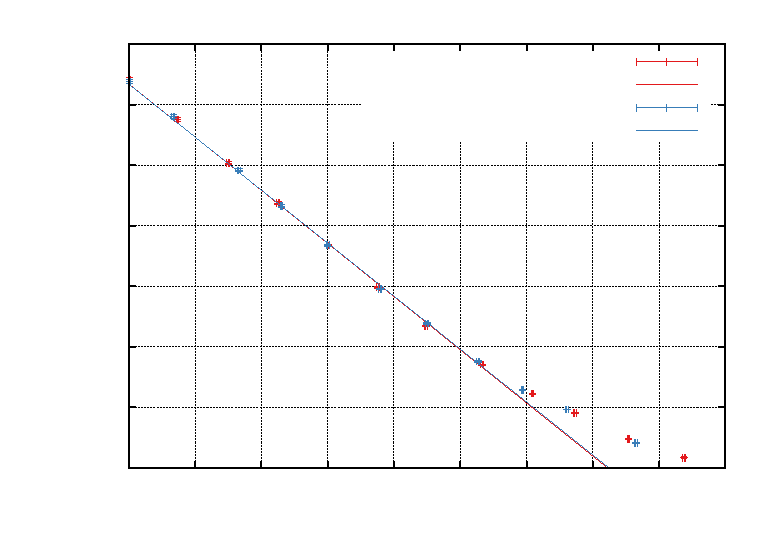
\includegraphics{./plots/photo/kennlinien_546nm}}%
    \gplfronttext
  \end{picture}%
\endgroup

	\caption{Kennlinien 546nm}
	\label{fig:kennlinien_546nm}
\end{figure}



% Messung 578nm
\begin{table}
	\centering
	\begin{subtable}{0.5\textwidth}
		\centering
		\vspace{0pt}
		\resizebox{0.95\columnwidth}{!}{%
			\begin{tabular}{SSS}
	\toprule
	{$U$ / \si{\volt}} & {$I-I_0$ / \si{\nano\ampere}} & {$\Delta (I-I_0)$ / \si{\nano\ampere}} \\
	\midrule
0.001 & 4.913 & 0.101 \\
0.055 & 4.253 & 0.087 \\
0.106 & 3.363 & 0.070 \\
0.161 & 2.623 & 0.055 \\
0.203 & 2.113 & 0.045 \\
0.239 & 1.753 & 0.037 \\
0.306 & 1.143 & 0.025 \\
0.351 & 0.813 & 0.019 \\
0.402 & 0.523 & 0.013 \\
0.459 & 0.303 & 0.008 \\
0.502 & 0.193 & 0.006 \\
0.557 & 0.103 & 0.004 \\
0.602 & 0.053 & 0.003 \\
0.651 & 0.023 & 0.003 \\
0.724 & 0.003 & 0.003 \\
	\bottomrule
\end{tabular}

		}
		\caption{Messung 1}
	\end{subtable}%
	\begin{subtable}{0.5\textwidth}
		\centering
		\vspace{0pt}
		\resizebox{0.95\columnwidth}{!}{%
			\begin{tabular}{SSS}
	\toprule
	{$U$ / \si{\volt}} & {$I-I_0$ / \si{\nano\ampere}} & {$\Delta (I-I_0)$ / \si{\nano\ampere}} \\
	\midrule
0.001 & 5.181 & 0.106 \\
0.048 & 4.371 & 0.090 \\
0.101 & 3.571 & 0.074 \\
0.150 & 2.951 & 0.061 \\
0.204 & 2.241 & 0.047 \\
0.260 & 1.661 & 0.036 \\
0.305 & 1.231 & 0.027 \\
0.356 & 0.821 & 0.019 \\
0.403 & 0.531 & 0.013 \\
0.445 & 0.351 & 0.009 \\
0.501 & 0.191 & 0.006 \\
0.542 & 0.121 & 0.005 \\
0.594 & 0.071 & 0.004 \\
0.642 & 0.031 & 0.003 \\
 & & \\
	\bottomrule
\end{tabular}

		}
		\caption{Messung 2}
	\end{subtable}

	\caption{Kennlinien der Photozelle f\"ur Licht der Wellenl\"ange $\lambda = \SI{578}{\nano\metre}$}
\end{table}

\begin{figure}
	\centering
	% GNUPLOT: LaTeX picture with Postscript
\begingroup
  \makeatletter
  \providecommand\color[2][]{%
    \GenericError{(gnuplot) \space\space\space\@spaces}{%
      Package color not loaded in conjunction with
      terminal option `colourtext'%
    }{See the gnuplot documentation for explanation.%
    }{Either use 'blacktext' in gnuplot or load the package
      color.sty in LaTeX.}%
    \renewcommand\color[2][]{}%
  }%
  \providecommand\includegraphics[2][]{%
    \GenericError{(gnuplot) \space\space\space\@spaces}{%
      Package graphicx or graphics not loaded%
    }{See the gnuplot documentation for explanation.%
    }{The gnuplot epslatex terminal needs graphicx.sty or graphics.sty.}%
    \renewcommand\includegraphics[2][]{}%
  }%
  \providecommand\rotatebox[2]{#2}%
  \@ifundefined{ifGPcolor}{%
    \newif\ifGPcolor
    \GPcolortrue
  }{}%
  \@ifundefined{ifGPblacktext}{%
    \newif\ifGPblacktext
    \GPblacktexttrue
  }{}%
  % define a \g@addto@macro without @ in the name:
  \let\gplgaddtomacro\g@addto@macro
  % define empty templates for all commands taking text:
  \gdef\gplbacktext{}%
  \gdef\gplfronttext{}%
  \makeatother
  \ifGPblacktext
    % no textcolor at all
    \def\colorrgb#1{}%
    \def\colorgray#1{}%
  \else
    % gray or color?
    \ifGPcolor
      \def\colorrgb#1{\color[rgb]{#1}}%
      \def\colorgray#1{\color[gray]{#1}}%
      \expandafter\def\csname LTw\endcsname{\color{white}}%
      \expandafter\def\csname LTb\endcsname{\color{black}}%
      \expandafter\def\csname LTa\endcsname{\color{black}}%
      \expandafter\def\csname LT0\endcsname{\color[rgb]{1,0,0}}%
      \expandafter\def\csname LT1\endcsname{\color[rgb]{0,1,0}}%
      \expandafter\def\csname LT2\endcsname{\color[rgb]{0,0,1}}%
      \expandafter\def\csname LT3\endcsname{\color[rgb]{1,0,1}}%
      \expandafter\def\csname LT4\endcsname{\color[rgb]{0,1,1}}%
      \expandafter\def\csname LT5\endcsname{\color[rgb]{1,1,0}}%
      \expandafter\def\csname LT6\endcsname{\color[rgb]{0,0,0}}%
      \expandafter\def\csname LT7\endcsname{\color[rgb]{1,0.3,0}}%
      \expandafter\def\csname LT8\endcsname{\color[rgb]{0.5,0.5,0.5}}%
    \else
      % gray
      \def\colorrgb#1{\color{black}}%
      \def\colorgray#1{\color[gray]{#1}}%
      \expandafter\def\csname LTw\endcsname{\color{white}}%
      \expandafter\def\csname LTb\endcsname{\color{black}}%
      \expandafter\def\csname LTa\endcsname{\color{black}}%
      \expandafter\def\csname LT0\endcsname{\color{black}}%
      \expandafter\def\csname LT1\endcsname{\color{black}}%
      \expandafter\def\csname LT2\endcsname{\color{black}}%
      \expandafter\def\csname LT3\endcsname{\color{black}}%
      \expandafter\def\csname LT4\endcsname{\color{black}}%
      \expandafter\def\csname LT5\endcsname{\color{black}}%
      \expandafter\def\csname LT6\endcsname{\color{black}}%
      \expandafter\def\csname LT7\endcsname{\color{black}}%
      \expandafter\def\csname LT8\endcsname{\color{black}}%
    \fi
  \fi
  \setlength{\unitlength}{0.0500bp}%
  \begin{picture}(7200.00,5040.00)%
    \gplgaddtomacro\gplbacktext{%
      \csname LTb\endcsname%
      \put(946,704){\makebox(0,0)[r]{\strut{} 0}}%
      \csname LTb\endcsname%
      \put(946,1518){\makebox(0,0)[r]{\strut{} 0.5}}%
      \csname LTb\endcsname%
      \put(946,2332){\makebox(0,0)[r]{\strut{} 1}}%
      \csname LTb\endcsname%
      \put(946,3147){\makebox(0,0)[r]{\strut{} 1.5}}%
      \csname LTb\endcsname%
      \put(946,3961){\makebox(0,0)[r]{\strut{} 2}}%
      \csname LTb\endcsname%
      \put(946,4775){\makebox(0,0)[r]{\strut{} 2.5}}%
      \csname LTb\endcsname%
      \put(1078,484){\makebox(0,0){\strut{} 0}}%
      \csname LTb\endcsname%
      \put(1794,484){\makebox(0,0){\strut{} 0.1}}%
      \csname LTb\endcsname%
      \put(2509,484){\makebox(0,0){\strut{} 0.2}}%
      \csname LTb\endcsname%
      \put(3225,484){\makebox(0,0){\strut{} 0.3}}%
      \csname LTb\endcsname%
      \put(3941,484){\makebox(0,0){\strut{} 0.4}}%
      \csname LTb\endcsname%
      \put(4656,484){\makebox(0,0){\strut{} 0.5}}%
      \csname LTb\endcsname%
      \put(5372,484){\makebox(0,0){\strut{} 0.6}}%
      \csname LTb\endcsname%
      \put(6087,484){\makebox(0,0){\strut{} 0.7}}%
      \csname LTb\endcsname%
      \put(6803,484){\makebox(0,0){\strut{} 0.8}}%
      \put(176,2739){\rotatebox{-270}{\makebox(0,0){\strut{}$\sqrt{I-I_0} \, / \, \si{\nano\ampere^{1/2}}$}}}%
      \put(3940,154){\makebox(0,0){\strut{}$U \, / \, \si{\volt}$}}%
      \put(3940,4665){\makebox(0,0){\strut{}}}%
    }%
    \gplgaddtomacro\gplfronttext{%
      \csname LTb\endcsname%
      \put(5816,4602){\makebox(0,0)[r]{\strut{}Messung 1}}%
      \csname LTb\endcsname%
      \put(5816,4382){\makebox(0,0)[r]{\strut{}Regressionsgerade 1}}%
      \csname LTb\endcsname%
      \put(5816,4162){\makebox(0,0)[r]{\strut{}Messung 2}}%
      \csname LTb\endcsname%
      \put(5816,3942){\makebox(0,0)[r]{\strut{}Regressionsgerade 2}}%
    }%
    \gplbacktext
    \put(0,0){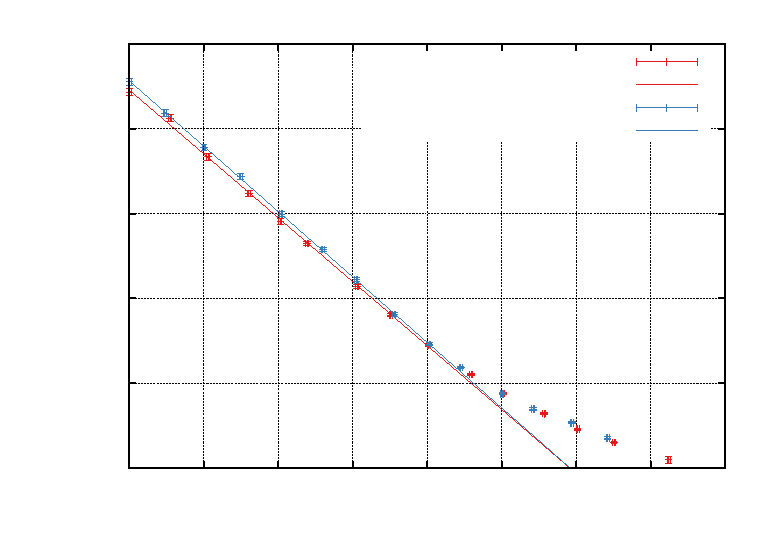
\includegraphics{./plots/photo/kennlinien_578nm}}%
    \gplfronttext
  \end{picture}%
\endgroup

	\caption{Kennlinien 578nm}
	\label{fig:kennlinien_578nm}
\end{figure}
